
\documentclass[a4paper]{article}
\usepackage[utf8]{inputenc}
\usepackage{amsmath}
\usepackage{amssymb,amsfonts,textcomp}
\usepackage[T1]{fontenc}
\usepackage[brazil]{babel}
\usepackage{color}
\usepackage{array}
\usepackage{hhline}
\usepackage{hyperref}
\usepackage[pdftex]{graphicx}
\usepackage{lipsum}  
\usepackage{float, natbib, verbatim} 

% Outline numbering
\setcounter{secnumdepth}{2}

% Page layout (geometry)
\setlength\voffset{-1in}
\setlength\hoffset{-1in}
\setlength\topmargin{1.0236in}
\setlength\oddsidemargin{0.9839in}
\setlength\textheight{9.0164995in}
\setlength\textwidth{6.3002996in}
\setlength\footskip{0.4327in}
\setlength\headheight{0.2362in}
\setlength\headsep{0.1965in}


% Pages styles
\makeatletter
\newcommand\ps@Standard{
\renewcommand\@oddhead{}
\renewcommand\@evenhead{}
\renewcommand\@evenfoot{\thepage}
\renewcommand\@oddfoot{\thepage}
\renewcommand\thepage{\arabic{page}}
}

% HEADER and FOOTER
\newcommand\ps@FirstPage{
\renewcommand\@oddhead{\itshape\small Modelos Lineares Generalizados ${\bullet}$  UFSM - Departamento de Estatística ${\bullet}$  17 de fevereiro de 2022}
\renewcommand\@evenhead{\@oddhead}
\renewcommand\@oddfoot{\itshape Modelo de Regressão Logística para compras realizadas a partir de anúncios na internet\hfill \thepage}
\renewcommand\@evenfoot{\@oddfoot}
\renewcommand\thepage{\arabic{page}}
}

%BIBLIOGRAFIA
\documentclass[letterpaper,10pt]{article}
\usepackage{biblatex} %Imports biblatex package
\addbibresource{ref.bib} %Import the bibliography file
%\printbibliography   colocar no fim do artigo

\begin{document}

\clearpage\setcounter{page}{1}%\pagestyle{Standard}
\thispagestyle{FirstPage} % header and footer first page

%%%%%%%%%%%%%%%%%%% Title %%%%%%%%%%%%%%%%%%%%

\begin{center}
	\begin{LARGE}
		\textbf{Modelo de Regressão Logística para compras realizadas a partir de anúncios na internet}
	\end{LARGE}
\end{center}

\bigskip

%%%%%%%%%%%% List of authors %%%%%%%%%%%%%%%
{\centering
João Inácio Scrimini\textsuperscript{1}\par  Joelmir Luz de Moura Junior\textsuperscript{1}\par}
\bigskip
{\centering
	1: Acadêmicos do Curso de Estatística da UFSM 	 \par}


\bigskip

%%%%%%%%%%%% Abstract %%%%%%%%%%%%\doublespacing

\hline
\bigskip
{\centering\bfseries\Large\color{black}Resumo 
	\par}
\smallskip

Este trabalho busca ajustar um modelo de Regressão Logística para avaliar as chances de ocorrências de compras a partir de anúncios na internet, onde como objetivo seja identificar qual o perfil do consumidor, buscando minimizar custos com marketing digital e direcionar produtos para os expecíficos clientes alvos. Assim, foi ajustado um modelo de Regressão Logística, com distribuição Bernoulli($\mu$) e função de ligação logística ($log\frac{\mu}{1-\mu}$), onde foi definido como variável dependente, se o cliente comprou ou não o produto, ao clicar no anúncio. E como variáveis independentes, gênero, idade e renda anual estimada. Por meio disso, foram realizados análises de diagnóstico e influência, para ajustes e "validação" do modelo. Com isso, aplicando o modelo final proposto em 12 clientes fictícios, concluindo que os indivíduos de maiores idades e melhores salários, tem chances maiores de realizar compras pelos anúncios na internet, independente do gênero.

\bigskip



%%%%%%%%%%%% Keywords %%%%%%%%%%%%
\textit{\textbf{Palavras-chave}: Função de ligação logística, distribuição Bernoulli, diagnóstico, influência, marketing digital. }

\bigskip
\hline


%%%%%%%%%%%% Body %%%%%%%%%%%%

\section{ Introdução}

\quad\ Em estudos estatísticos, é muito relevante analisar a relação entre variáveis, especialmente a influência que uma ou mais variáveis explicativas têm sobre uma variável resposta. Neste sentido os estudos de Modelos Lineares Generalizados (MLG) servem para fazer esta associação onde até então, os modelos lineares mais comumente utilizado, não se mostravam mais tão eficientes, por exigirem a confirmação de uma série de suposições para sua validação.

Os MLGs então, podem ser entedidos como uma extensão dos modelos de regressão linear, pois além de tudo, expandem as suposições admitidas e desta forma podemos modelar variáveis que assumem a forma de contagem, categóricas e binárias, como no caso do nosso estudo. No momento em que nos foi proposto este trabalho, decidimos por interpretar um banco de dados que determina se um usuário comprou um produto específico ou não, através de uma propaganda na internet. Utilizaremos então a regressão logística na modelagem deste fenômeno devido a peculiaridade da nossa variável resposta, que assume valores 0 ou 1, sendo 1 a compra do produto. Este estudo se faz relevante pois auxilia na montagem do perfil do consumidor em que se quer atingir com os anúncios e desta forma, minimizar os custos com publicidade. Ao atingir o público de interesse, com maiores chances de compra para certo produto, o vendedor pode criar anúncios direcionados sem que precise testar isto empíricamente. Assim, este trabalho tem como objetivo ajustar um modelo de Regressão Logística para avaliar as chances de ocorrências de compras a partir de anúncios na internet, identificando o perfil do consumidor.

Para fins de melhor organizar as ideias propostas, o artigo está separado em cinco seções, sendo, Introdução a primeira, como forma de ambientar o leitor ao estudo o qual iremos discorrer ao longo do trabalho; Referencial Teórico, que serve tanto para confirmar conceitos utilizados no estudo, como familiarizar o leitor a respeito deles; Análise do modelo de Regressão Logística, seção onde estão as principais análises do modelo, dividídos em duas subseções, sendo a primeira, variáveis em estudo e na segunda, análise de diagnóstico e influência; Predição, seção contendo a aplicação do modelo final proposto em outros indíviduos; Por fim, as conclusões do estudo realizado.


\section{Referencial Teórico}

\quad \ Para introduzirmos o assunto dos Modelos Lineares Generalizados, devemos abordar a família exponencial, pois o mesmo pressupõe que a variável resposta tenha essa distribuição. 

\subsection{Família exponencial}
\quad \ Segundo \cite{Turkman} uma variável aleatória Y segue uma distribuição da família exponencial caso sua função densidade de probabilidade puder ser descrita da seguinte forma:
\begin{equation*}
    f(y_i|\theta_i,\phi) = exp[\phi\left\{y_i\theta_i-b(\theta_i)\right\}+c(y_i,\phi)]
\end{equation*}
\quad \ Onde $\phi$ é o parâmetro de precisão. Neste caso, distribuições pertencentes à família exponencial, são de interesse do estudo.

\subsection{Distribuição de Bernoulli}
\quad \ A Distribuição de Bernoulli é uma distribuição discreta com espaço amostral $\Omega=\left\{0,1\right\}$, onde p assume o valor 1 sendo o sucesso ou 0 sendo o fracasso para o evento. Sua função de probabilidade é dada por:
\begin{equation*}
f(k,p)= \left\{ \begin{array}{ll} p, & k=1\\
0, & \mbox{ caso contrario}.\end{array} \right.
\end{equation*}
\quad \ No caso do nosso estudo, optamos por utilizar esta distrbuição devido a variável resposta assumir apenas valores 1 ou 0. Sendo o sucesso, o usuário que realizou uma compra através de um anúncio da internet, equanto o 0 seria o usuário que não realizou.

\subsection{Componente aleatório}
\quad \ Dado um conjunto de variáveis aleatórias independentes $Y_i$ com $i=1,...,n$ com distribuição pertencente à \textit{família exponencial} e $E(Y_i)=\mu_i$ para $i=1,...,n$ onde $\phi>0$ é um parâmetro de dispersão constante ou variável.

\subsection{Componente sistemático}
\quad \ As variáveis explicativas entram na forma de uma estrutura linear de seus efeitos da seguinte forma:
\begin{equation*}
    \eta_i=\sum_{j=1}^nx_{ij}\beta_i
\end{equation*}
onde $\beta=(\beta_1,...,\beta_k)^T$é o vetor de parâmetros e $\eta=(\eta_1,...,\eta_k)^T$ é o preditor linear.

\subsection{Função de Ligação}
\quad \ A função que relaciona o componente aleatório $Y$ ao componente sistemático $\eta$ é denominada "Função de Ligação", que tem a seguinte forma: $\eta_i=g(\mu_i)$, sendo esta uma função monótona e duplamente diferenciável. Esta função varia conforme o espaço paramétrico de $\mu$ e da distribuição. As mais usuais são:
\begin{itemize}
    \item Potência:$\eta = \mu\lambda$, para um determinado $\lambda \in \mathbb{R}$;simbolo de pertence no latex
    \item Logarítmica: $\eta$= log $\mu$, para $\mu \in \mathbb{R}^*$;
    \item Logística: $\eta=log(\frac{\mu}{1-\mu})$, para um determinado $\mu \in (0,1)$;
    \item Probit: $\eta=\phi^-1(\mu)$, em que $\phi(.)$ é a função de distribuição acumulada da normal padrão.
\end{itemize}


\section{Análise do modelo de Regressão Logística}

\subsection{Variáveis em estudo}

\quad \ O presente estudo tem como referência o banco de dados de compras em anúncios, disponível em \cite{kaggle}, com 400 observações, sendo elas os clientes que entraram no anúncio, contendo 4 variáveis, apresentadas na tabela \ref{tab1}, onde Comprado é a variável de desfecho. 

\begin{table}[H] 
\caption{Variáveis do estudo sobre compras em sites.}
\begin{center}
\begin{tabular}{ll}
\hline
 Variável & Descrição\\
 \hline
Idade & Idade dos clientes que entraram no anúncio\\
Salário & Salário anual estimado dos clientes que entraram no anúncio\\
Comprado & Classificação 0 ou 1, sendo 1 realizado a compra e 0 não realizado a compra\\
Gênero & Classificação 0 ou 1, sendo 1 feminino e 0 masculino\\
\hline
\end{tabular}
\label{tab1}
\end{center}
\end{table}

Na tabela \ref{tab2} é apresentado as medidas descritivas das variáveis em estudo, onde a idade média dos clientes foram, aproximadamente, de 38 anos, mínima de 18 anos e máxima de 60 anos. O salário médio anual apresentou-se em 69743 mil, mínimo de 15000 mil e máximo de 150000 mil. Para Gênero foram divididos em masculino e feminino, sendo 196 homens e 204 mulheres, recebendo 0 para masculino e recebendo 1 para feminino, representando média de $51\%$  de mulheres. E Comprado para a variável de desfecho, recebendo 1 ou 0, quando comprado ou não comprado, respectivamente, representando média de  $36\%$ de clientes que realizaram a compra.
\begin{table}[H] 
\caption{Análise descritiva dos dados em estudo.}
\begin{center}
\begin{tabular}{lrrrrrr}
\hline
 Variável & Mínimo & 1º Quantil & Mediana & Média & 3º Quantil & Máximo\\
 \hline
Idade & 18.00 & 29.75 & 37.00 & 37.66 & 46.00 & 60.00\\
Salário & 15000 & 43000 & 70000 & 69743 & 88000 & 150000\\
Comprado & 0.00 & 0.00 & 0.00 & 0.36 & 1.00 & 1.00\\
Gênero & 0.00 & 0.00 & 1.00 & 0.51 & 1.00 & 1.00\\
\hline
\end{tabular}

\label{tab2}
\end{center}
\end{table}

Portanto, com as descrições das variáveis e as análises descritivas, presentes nas tabelas \ref{tab1} e \ref{tab2}, foi identificado que o melhor ajuste de modelo seria por regressão logística, onde a distribuição utilizada é a Bernoulli($\mu$), que assume valores 0 ou 1, como a variável de desfecho desse estudo. Com isso, a função de ligação utilizada foi a logística ($log\frac{\mu}{1-\mu}$), com o intuíto de estimar a probabilidade de uma pessoa clicar em um anúncio e realizar a compra do produto. Assim, temos o primeiro modelo para análise.

%Modelo inicial
Modelo inicial com função de ligação logística, $g(x) = log\frac{\mu}{1-\mu}$: 

\begin{equation}\label{eq:1}
g(x)= \beta_0 + \beta_1 x_1  + \beta_2 x_2+ \beta_3 x_3
\end{equation}
em que $Y \sim Bernoulli(\mu)$, onde $ P(Y=1)=\mu$, $x_1$ = Idade, $x_2$= Gênero e $x_3$= Salário.

No modelo inicial \ref{eq:1} somente a variável Gênero ($x_1$) não apresentou significância, conforme vemos na tabela \ref{tab3}, mostrando o ajuste desse modelo. O modelo apresentou coeficiente de determinação ($R^2$) de $63\%$, onde representa a quantidade explicativa do modelo nos dados, e o critério de informação de Akaike ($AIC$) de $283.84$, que representa um critério de seleção de modelo, buscando minimizar a perda de informação. Portanto, como $x_1$ não foi significativo, será retidado do modelo, pelo método de Backward, que é indicado quando existem poucas cováriaveis. No qual, consiste em retirar covariáveis uma por uma, quando não apresentam significância, sendo primeiramente retiradas as covariáveis com maiores p-valores (ou que minimizem o AIC), até que permaneçam no modelo só covariáveis significativas. Assim, apresentado na tabela \ref{tab4} esse primeiro ajuste realizado, retirando
a cováriavel Gênero. Percebe-se que todas as cováriaveis e intercepto foram significativos, podendo seguir para as análises de diagnóstico e influência do modelo. 

Na tabela \ref{tab3} são apresentados os resultados 
\begin{table}[H] 
\caption{Coeficientes do modelo inicial.}
\begin{center}
\begin{tabular}{lrrrrl}
\hline
  & Estimativa ($\beta$'s) & Erro Padrão & Estatística Z & P-valor(>|z|)\\
\hline
(Intercepto) & -12.4497907 & 1.3091557 & -9.509786 & < 2e-16 & ***\\
Idade & 0.2369694 & 0.0263771 & 8.983922 & < 2e-16 & ***\\
Gênero & -0.3338434 & 0.3052264 & -1.093757 & 0.274 &\\
Salário & 0.0000364 & 0.0000055 & 6.658530 & 2.77e-11 & ***\\
\hline
\end{tabular}
\\\tiny{\hspace{-5cm} Código de significância: $0\ ^{***}\ 0.001\ ^{**}\ 0.01\ ^{*}\ 0.05\ ^{.}\ 0.1 \ 1$}
\label{tab3}
\end{center}
\end{table}


\begin{table}[H] 
\caption{Coeficientes do modelo com primeiro ajuste.}
\begin{center}
\begin{tabular}{lrrrrl}
\hline
  & Estimativa ($\beta$'s) & Erro Padrão & Estatística Z & P-valor(>|z|)\\
\hline
(Intercepto) & -12.4339881 & 1.2997812 & -9.566216 & < 2e-16 & ***\\
Idade & 0.2334894 & 0.0259062 & 9.012886 & < 2e-16 & ***\\
Salário & 0.0000359 & 0.0000054 & 6.612700 & 3.77e-11 & ***\\
\hline
\end{tabular}
\\\tiny{\hspace{-5cm} Código de significância: $0\ ^{***}\ 0.001\ ^{**}\ 0.01\ ^{*}\ 0.05\ ^{.}\ 0.1 \ 1$}
\label{tab4}
\end{center}
\end{table}

\subsection{Análise de diagnóstico e influência}
\quad \ Sendo assim, vamos para a análise de influência,  buscando identificar possíveis observações influentes no ajuste do modelo. Para isso, na figura \ref{fig:alav1} é apresentado o gráfico de alavancagem, sendo um dos testes considerados na análise de influência, que consiste em identificar pontos de alavancagem, com valores atípicos no espaço das variáveis explicativas, podendo, não necessáriamente serem pontos de influência. No qual, deverão ser retirados e testados, verificando suas inflências nas estimatimas e correspondentes erros padrões. Dessa forma, nota-se no gráfico que existem várias possíveis observações influêntes, com valores atípicos dos demais.


\begin{figure}[H] 
    \centering % para centralizar a imagem na página
    \caption{Gráfico de alvancagem}
    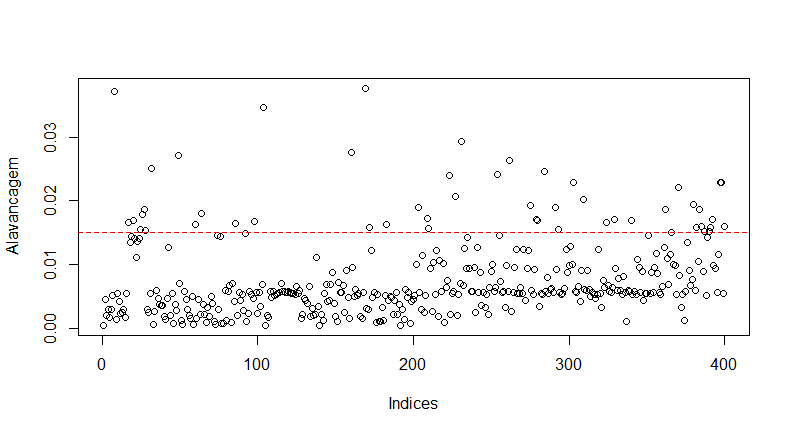
\includegraphics[width=0.9\textwidth]{imagens/Alav1.png}
    \label{fig:alav1}
\end{figure}

Na figura \ref{fig:cook1} é apresentado o gráfico da distância de Cook, da mesma forma que foi visto na alavancagem, algumas observações podem exercer influência sobre as estimativas dos parâmetros e estatísticas utilizadas, conforme suas disposições de pontos no espaço das variavéis. Com isso, nota-se que existem observações muito influentes vizualmente, com valores muito atípicos dos demais, podendo mudar consideravelmente as estimativas do modelo.

\begin{figure}[H] 
    \centering % para centralizar a imagem na página
    \caption{Gráfico de distância de Cook}
    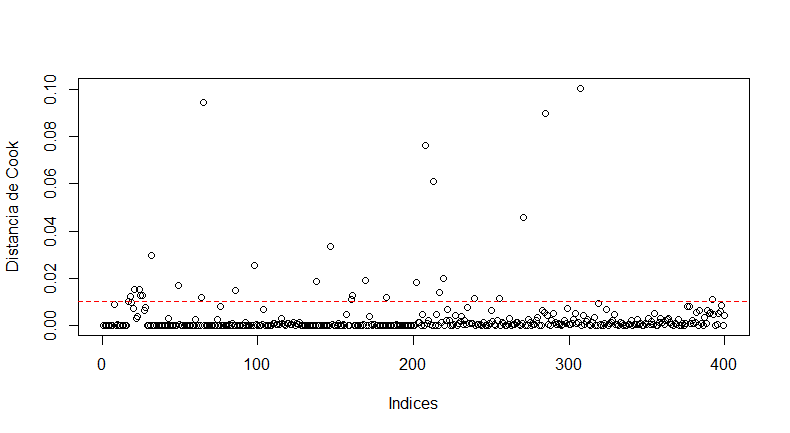
\includegraphics[width=0.9\textwidth]{imagens/Cook1.png}
    \label{fig:cook1}
\end{figure}

Na figura \ref{fig:res1} é apresentado o gráfico dos resíduos, percebe-se que existem várias observações que não estão presentes dentro dos limites, a maioria dessas observações foram identificadas como as mesmas observações presentes na figura \ref{fig:cook1}, com maiores valores atípicos.

\begin{figure}[H] 
    \centering % para centralizar a imagem na página
    \caption{Gráfico dos resíduos}
    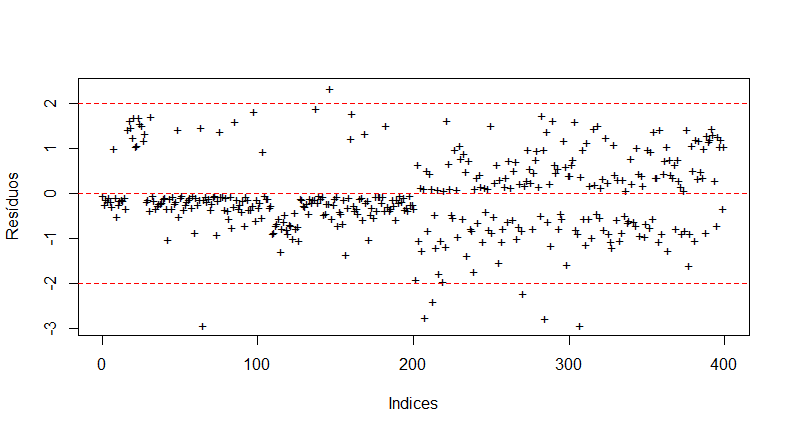
\includegraphics[width=0.9\textwidth]{imagens/Res1.png}
    \label{fig:res1}
\end{figure}

Na figura \ref{fig:es1} é apresentado o envelope simulado baseado nos resíduos de desvio, que facilita a vizualização de outliers, observações que não se encontram destro das bandas de conficança, ou seja, observações que não se ajustam ao modelo e se distanciam das demais.  No gráfico, nota-se que existe uma grande quantidade de observações fora das bandas de confiança, principalmente em suas extremidades, podendo serem influênciados pelas observações atípicas vizualidadas nos gráficos anteriores de testes de influência.
\begin{figure}[H] 
    \centering % para centralizar a imagem na página
    \caption{Gráfico do envelope simulado baseado nos resíduos de desvio}
    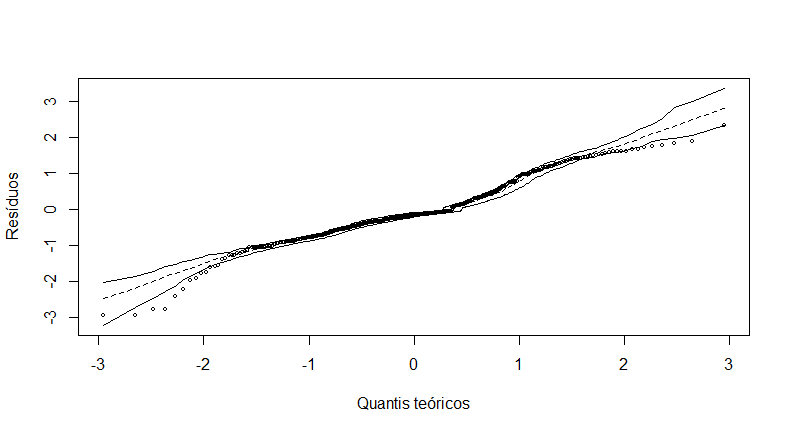
\includegraphics[width=0.9\textwidth]{imagens/ES1.png}
    \label{fig:es1}
\end{figure}
A apartir dos testes e análises realizados, foi identificado a necissidade de retirar do modelo inicial algumas observações que mostravam-se muito influentes, sendo elas os respectivos clientes: 32, 65, 98, 138, 147, 161, 202, 208, 213, 217, 219, 239, 255, 271, 285, 299, 307 e 377. Estes 18 clientes, apresentaram valores não condizentes aos demais, para as variáveis em estudo, não se ajustando ao modelo proposto. Portanto o modelo foi ajustado sem essas 18 observações dos clientes, considerando agora uma amostra de 382 clientes.

Como essas observações retiradas podem afetar a exclusão ou aceitação de alguma covariável, foi verificado novamente pelo modelo inicial (\ref{eq:1}). Assim, temos na tabela \ref{tab5} os coeficientes desse ajuste. Nota-se uma grande diferença nas estimativas dos parametros ($\beta's$) e nenhuma alteração na significância das cováriaveis, mantendo Gênero  não significativo. Sendo retirado novamente do modelo, pelo metódo de Backward, como vemos no reajuste pela tabela \ref{tab6}, com todas covariáveis e intercepto significativos, passando o modelo a ter medidas de $AIC$ de $165.14$ e $R^2$ de $80.86\%$. Portanto, serão apresentados as medidas de influência desse segundo ajuste do modelo, que é apresentado pela tabela \ref{tab6}, verificando novas possíveis influências.
%Modelo final ajustado 

\begin{table}[H] 
\caption{Coeficientes do modelo inicial sem observações influentes.}
\begin{center}
\begin{tabular}{lrrrrl}
\hline
  & Estimativa ($\beta$'s) & Erro Padrão & Estatística Z & P-valor(>|z|)\\
\hline
(Intercepto) & -28.1983223 & 3.8424838 & -7.3385664 & < 2.16e-13 & ***\\
Idade & 0.5515104 & 0.0755366 & 7.3012316 & < 2.85e-13 & ***\\
Gênero & 0.3907976 & 0.4061205 & 0.9622699 & 0.336 &\\
Salário & 0.0000775 & 0.0000120 & 6.4521757 & 1.10e-10 & ***\\
\hline
\end{tabular}
\\\tiny{\hspace{-5cm} Código de significância: $0\ ^{***}\ 0.001\ ^{**}\ 0.01\ ^{*}\ 0.05\ ^{.}\ 0.1 \ 1$}
\label{tab5}
\end{center}
\end{table}


\begin{table}[H] 
\caption{Coeficientes do modelo com segundo ajuste.}
\begin{center}
\begin{tabular}{lrrrrl}
\hline
  & Estimativa ($\beta$'s) & Erro Padrão & Estatística Z & P-valor(>|z|)\\
\hline
(Intercepto) & -27.4851628 & 3.6890903 & -7.450390 & < 9.31e-14 & ***\\
Idade & 0.5416994 & 0.0734791 & 7.372152 & < 1.68e-13 & ***\\
Salário & 0.0000759 & 0.0000117 & 6.474322 & 9.52e-11 & ***\\
\hline
\end{tabular}
\\\tiny{\hspace{-5cm} Código de significância: $0\ ^{***}\ 0.001\ ^{**}\ 0.01\ ^{*}\ 0.05\ ^{.}\ 0.1 \ 1$}
\label{tab6}
\end{center}
\end{table}

Nas análises de influência, percebe-se no gráfico de alavancagem mostrado pela figura \ref{fig:alav2}, que existem algumas observações um pouco mais atípicas, nas quais, poderiam ser possíveis influentes. Sendo uma delas a observação 169, apresentando maior índice de alavanca. Na qual, foi verificada, sendo retidada do modelo, mas não apresentou influência.

\begin{figure}[H] 
    \centering % para centralizar a imagem na página
    \caption{Gráfico de alvancagem}
    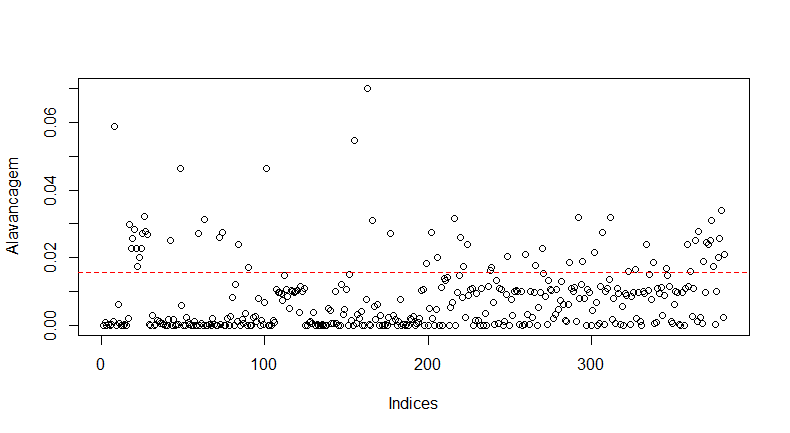
\includegraphics[width=0.9\textwidth]{imagens/Alav2.png}
    \label{fig:alav2}
\end{figure}


Na figura \ref{fig:cook2} é apresentado o gráfico da distância de Cook, onde vemos que mesmo existindo algumas observações fora do limite, elas não apresentam uma indicação de outliers, sendo de pouca influência no modelo.
\begin{figure}[H] 
    \centering % para centralizar a imagem na página
    \caption{Gráfico de distância de Cook}
    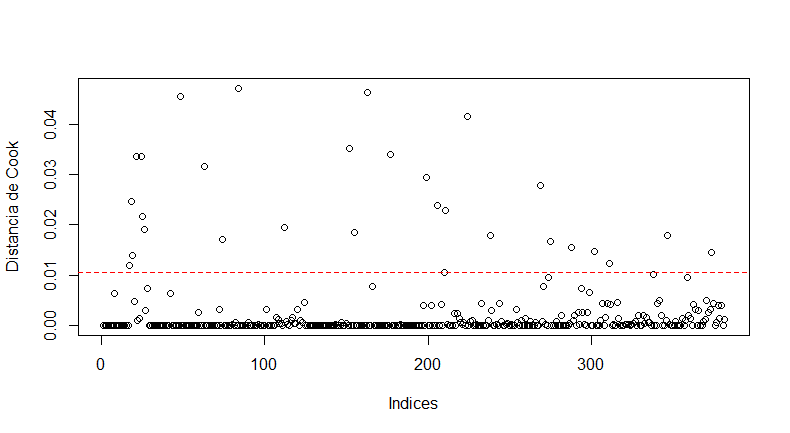
\includegraphics[width=0.9\textwidth]{imagens/Cook2.png}
    \label{fig:cook2}
\end{figure}


Pelo gráfico dos resíduos, apresentado pela figura \ref{fig:res2}, percebe-se que praticamente todas as observações estão presentes dentro dos limites. Onde, conseguimos vizualizar uma melhora significativa no envelope simulado, apresentado na figura \ref{fig:es2}, contendo praticamente todas as observações dentro das bandas de confiança de $95\%$. Com isso, indicando um bom ajuste no modelo proposto. 
\begin{figure}[H] 
    \centering % para centralizar a imagem na página
    \caption{Gráfico dos resíduos}
    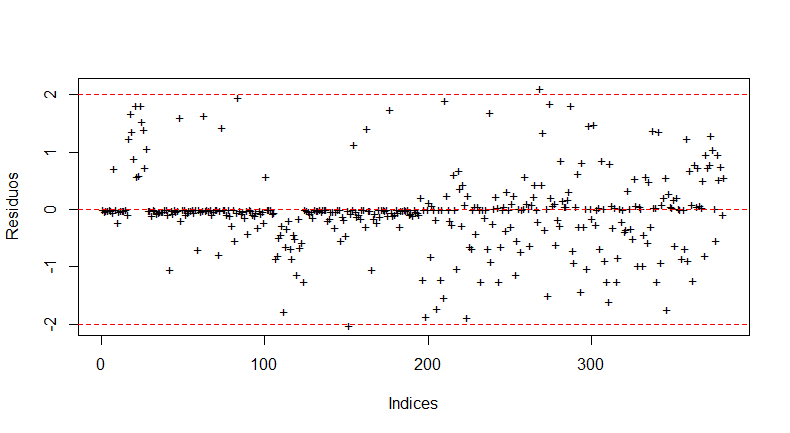
\includegraphics[width=0.9\textwidth]{imagens/Res2.png}
    \label{fig:res2}
\end{figure}


\begin{figure}[H] 
    \centering % para centralizar a imagem na página
    \caption{Gráfico do envelope simulado baseado nos resíduos de desvio}
    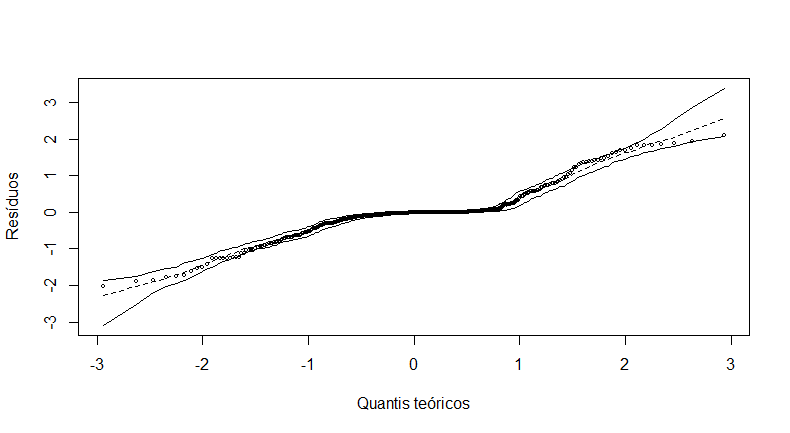
\includegraphics[width=0.9\textwidth]{imagens/ES2.png}
    \label{fig:es2}
\end{figure}
Portanto, como nenhuma outra observação se mostrou influente, manteremos o segundo ajuste realizado no modelo, apresentado na tabela \ref{tab6}. Assim, o modelo final proposto é apresentado abaixo:

Modelo ajustado com função de ligação logistica, $g(x) = log\frac{\mu}{1-\mu}$: 

\begin{equation}\label{eq:2}
g(x)= -27.49 + 0.54 x_1 + 7.59e^{-5} x_3
\end{equation}
em que $Y \sim Bernoulli(\mu)$, onde $ P(Y=1)=\mu$, $x_1$ = Idade e $x_3$= Salário. Com medidas de $AIC$ de $165.14$ e $R^2$ de $80.86\%$.


\section{Predição}

\quad \ Nesta seção, análisaremos a efetividade do modelo final proposto (\ref{eq:2}), onde verificaremos a probabilidade de diferentes possíveis clientes realizarem compras em anúncios na internet, com o intuíto de criar um perfil do consumidor alvo, por meio da idade ($x_1$) e salário anual estimado ($x_3$). Para a obtenção da probabilidade de compras de um indíviduo em anúncios na internet, $E(Y)$, é necessário aplicar uma função inversa a função de ligação, representado a seguir:

\begin{equation}\label{eq:3}
E(Y) = \frac{e^{g(x)}}{1+e^{g(x)}},
\end{equation}
em que g(x) é a função de ligação, representado pelo modelo final proposto (\ref{eq:2}).

Portanto, o modelo final proposto (\ref{eq:2}) foi aplicado por meio da função apresentada em (\ref{eq:3}), prevendo as chances de compras em anúncios na internet, apresentados na tabela \ref{tab7}, onde foram testados $12$ indivíduos ficticios de diferentes idades e sálarios. Assim, nota-se que a maior chance de compra entre esses clientes fictícios, foi no indívíduo 8, sendo uma pessoa de $60$ anos, com salário anual de $15000$ mil, apresentando probabilidade de compra, aproximadamente, de $99.76\%$. O indivíduo 1, com idade de $20$ anos e salário de $40000$ mil, apresentou a menor probabilidade, sendo, aproximadamente, de $0.0001\%$. Também, pode-se notar que a cováriavel idade é mais influente na variável dependente, mostrando que quanto maior a idade do cliente, maiores as chances de compras. Para o salário, acaba sendo bem pouco influente, mas mesmo assim, clientes com salários maiores tem chances de compras um pouco melhores.

\begin{table}[H] 
\caption{Aplicação do modelo final proposto em outros possíveis clientes.}
\begin{center}
\begin{tabular}{lrrr}
\hline
 Cliente & Idade & Salário & Prob. de compra ($\%$)\\
 \hline
Indivíduo 1 & 20 & 40000 & 0.0001\\
Indivíduo 2 & 30 & 40000 & 0.0260\\
Indivíduo 3 & 40 & 40000 & 5.4474\\
Indivíduo 4 & 45 & 40000 & 46.1576\\
Indivíduo 5 & 50 & 40000 & 92.7304\\
Indivíduo 6 & 20 & 120000 & 0.0509\\
Indivíduo 7 & 40 & 120000 & 96.1506\\
Indivíduo 8 & 60 & 15000 & 99.7644\\
Indivíduo 9 & 50 & 15000 & 65.6672\\
Indivíduo 10 & 45 & 15000 & 11.3901\\
Indivíduo 11 & 30 & 100000 & 2.4127\\
Indivíduo 12 & 35 & 80000 & 7.4607\\
\hline
\end{tabular}
\label{tab7}
\end{center}
\end{table}

\section{Conclusão}

\quad \ Este artigo teve por finalidade ajustar um modelo linear, buscando avaliar as chances de compras em anúncios na internet, verificando o perfil do consumidor alvo. Para isso, foi identificado que o melhor MLG para esse trabalho seria pela regressão logística, por conter como variável dependente, a variável Comprado, onde assume 0 ou 1, quando 1 efetuada a compra de determidado produto, podendo verificar as chances de compras dos possíveis clientes. Assim, o modelo foi ajustado por regressão logística, onde assume distribuição Bernoulli($\mu$) e função de ligação logística ($log\frac{\mu}{1-\mu}$), para a validação desse modelo, foram realizados análises de diagnóstico e influência, buscando possíveis observações influentes nos dados, e o  método de Backward, para exclusão de covariáveis não significativas. por fim, aplicando uma função inversa a função de ligação logística, para realizar as predições de chances de compras.

Com isso, foram retiradas do modelo 18 observações que apresentaram influências, sendo elas os clientes: 32, 65, 98,138, 147, 161, 202, 208, 213, 217, 219, 239, 255, 271, 285, 299, 307 e 377, presentes no banco de dados. Sendo retirado pelo método de Backward, a covariável Gênero, por não conter significância no modelo. Assim, o modelo final proposto (\ref{eq:2}), apresentou $AIC$ de $165.14$ e $R^2$ de $80.86\%$. 

Pelas predições realizadas, observou-se que indívios de maiores idades, acabam sendo mais influenciados pelos anúncios na internet, tentendo a realizarem mais compras que uma pessoa mais jovem, mesmo podendo conter menor aquisição financeira, ou seja, menor salário. Assim, pessoas mais jovens e independentemente da aquisição financeira, não tendem a realizarem muitas compras por anúncio, até por motivos da maioria apresentarem menores rendas e menor estabilidade financeira, supõe-se que acabam entrando no anúncio mais por curiosidade. Já, pessoas de maior idade, supõe-se que entram no anúncio por interesse, logo aumentando muito as chances de compras. Assim, o público alvo de anúncios na internet, foi identificado como indivíduos de maiores idades e com melhores salários, independente do gênero.

\printbibliography 
Gauss Moutinho Cordeiro e Clarice GB Demétrio. “Modelos lineares generalizados e extensões”. Em:
Piracicaba: USP (2008).



\end{document}
